\documentclass{esannV2}
\usepackage[dvips]{graphicx}
\usepackage[latin1]{inputenc}
\usepackage{amssymb,amsmath,array}

\usepackage{xcolor}
\usepackage{hyperref}
\urlstyle{same}

%
\voffset 0 cm \hoffset 0 cm \addtolength{\textwidth}{0cm}
\addtolength{\textheight}{0cm}\addtolength{\leftmargin}{0cm}


\begin{document}
%style file for ESANN manuscripts
\title{Few-shot on Federated Learning}

%***********************************************************************
% AUTHORS INFORMATION AREA
%***********************************************************************

\author{Anna Mosolova$^1$, Elisa Lubrini$^1$ and Christophe Cerisara$^2$ 

% DO NOT MODIFY THE FOLLOWING '\vspace' ARGUMENT
\vspace{.3cm}\\
%
% Addresses and institutions (remove "1- " in case of a single institution)
1- Universite de Lorraine - IDMC \\
Pole Herbert Simon, 13 Rue Michel Ney, 54000 Nancy - France
%
% Remove the next three lines in case of a single institution
\vspace{.1cm}\\
2- Inria - Dept of Second Author \\
Address of Second Author's school - France\\
}
%***********************************************************************
% END OF AUTHORS INFORMATION AREA
%***********************************************************************

\maketitle

\begin{abstract}
Current restrictions on confidentiality often prevent data from leaving personal devices and being sent to a central server on which a central model is trained. The problem of machine learning being hindered by scarcity of data can be tackled using few-shot learning (FSL) techniques. In this paper we explore the a possible application of few-shot learning to a federated dataset, where each node (or device) only holds a very limited amount of data. Our experiments are carried out using Google's T5 model, which is designed to perform well on data-scarce tasks. The results of a few experiments are reported, together with a brief summary of our findings.
\end{abstract}

\section{Introduction}
\textcolor{green}{\textbf{[...]}}

\subsection{Federated learning}
Federated learning is a technique that has been raising in popularity since it was first introduced by Google in 2016. The concept behind federated learning is that of training models on users' devices so that service providers can benefit from a model that has full access to private data, without the need for them to access such data directly.

\subsection{Few-shot learning}
Few-shot learning is a machine learning method used to generalise to a new task based on prior knowledge of other tasks \cite{wang2020generalizing}. It is mainly used when limited data is available \textcolor{green}{\textbf{[...]}}

\subsection{Related work}
According to our knowledge, no experiments have been published so far applying few-shot learning to federated datasets. 
\textcolor{green}{\textbf{[...]}}

\section{Method}
Our experiments will consist in the application of few shot learning on two datasets for sentiment analysis. The first, Amazon Review \cite{keung2020multilingual} has proven to perform well with few-shot learning and will be separated into nodes which each represent a device in a federated setting. The second, Sent140 \cite{caldas2019leaf}, is a federated dataset composed of Twitter comments, where each user corresponds to a node. We will use Google's T5 model, which is designed to perform well on tasks for which data is particularly scarce. Our results will then be compared with the current benchmark for each dataset \textcolor{green}{\textbf{\cite{Bench1}}} \textcolor{green}{\textbf{\cite{Bench2}}}
 
\subsection{Text-To-Text Transfer Transformer}
Text-To-Text Transfer Transformer (T5) \cite{t5} is a language model with a text-to-text framework where the input consists in the description of the task and the data on which the task is to be carried out.

\begin{figure}[h]
\begin{center}
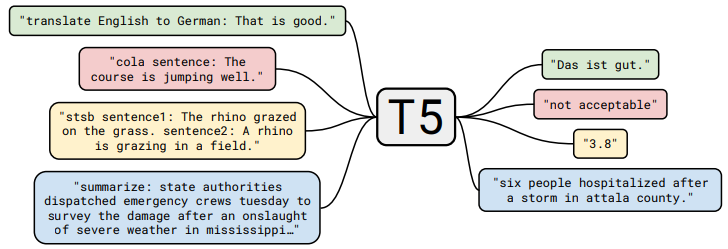
\includegraphics[width=\textwidth]{pics/T5.png}
\caption{T5 input and output examples, as illustrated in the original paper \cite{t5}.}
\label{fig:user}
\end{center}
\end{figure}

\subsection{Datasets}
The Multilingual Amazon Review Corpus (MARC) \cite{keung2020multilingual} \textcolor{green}{\textbf{[...]}}


Sent140 \cite{caldas2019leaf} is a federated dataset whose tweets are automatically annotated based on the emoticons present in them. Each device is represented by a different twitter user.

\section{Experiments}
\textcolor{green}{\textbf{[...]}}

\section{Results}
\textcolor{green}{\textbf{[...]}}

\section{Conclusion}
\textcolor{green}{\textbf{[...]}}


% ****************************************************************************
% BIBLIOGRAPHY AREA
% ****************************************************************************

\begin{footnotesize}

\bibliographystyle{unsrt}
\bibliography{bib.bib}

\end{footnotesize}

%\documentclass{esannV2}
\usepackage[dvips]{graphicx}
\usepackage[latin1]{inputenc}
\usepackage{amssymb,amsmath,array}

\usepackage{hyperref}
\urlstyle{same}

%***********************************************************************
% !!!! IMPORTANT NOTICE ON TEXT MARGINS !!!!!
%***********************************************************************
%
% Please avoid using DVI2PDF or PS2PDF converters: some undesired
% shifting/scaling may occur when using these programs
% It is strongly recommended to use the DVIPS converters, and to submit
% PS file. You may submit a PDF file if and only if you use ADOBE ACROBAT
% to convert your PS file to PDF.
%
% Check that you have set the paper size to A4 (and NOT to letter) in your
% dvi2ps converter, in Adobe Acrobat if you use it, and in any printer driver
% that you could use.  You also have to disable the 'scale to fit paper' option
% of your printer driver.
%
% In any case, please check carefully that the final size of the top and
% bottom margins is 5.2 cm and of the left and right margins is 4.4 cm.
% It is your responsibility to verify this important requirement.  If these margin requirements and not fulfilled at the end of your file generation process, please use the following commands to correct them.  Otherwise, please do not modify these commands.
%
\voffset 0 cm \hoffset 0 cm \addtolength{\textwidth}{0cm}
\addtolength{\textheight}{0cm}\addtolength{\leftmargin}{0cm}

%***********************************************************************
% !!!! USE OF THE esannV2 LaTeX STYLE FILE !!!!!
%***********************************************************************
%
% Some commands are inserted in the following .tex example file.  Therefore to
% set up your ESANN submission, please use this file and modify it to insert
% your text, rather than staring from a blank .tex file.  In this way, you will
% have the commands inserted in the right place.

\begin{document}
%style file for ESANN manuscripts
\title{Few-shot on Federated Learning}

%***********************************************************************
% AUTHORS INFORMATION AREA
%***********************************************************************

\author{Anna Mosolova$^1$, Elisa Lubrini$^1$ and Christophe Cerisara$^2$ 

%
% Optional short acknowledgment: remove next line if non-needed
%\thanks{This is an optional funding source acknowledgement.}
%
% DO NOT MODIFY THE FOLLOWING '\vspace' ARGUMENT
\vspace{.3cm}\\
%
% Addresses and institutions (remove "1- " in case of a single institution)
1- Universite de Lorraine - IDMC \\
Pole Herbert Simon, 13 Rue Michel Ney, 54000 Nancy - France
%
% Remove the next three lines in case of a single institution
\vspace{.1cm}\\
2- Inria - Dept of Second Author \\
Address of Second Author's school - France\\
}
%***********************************************************************
% END OF AUTHORS INFORMATION AREA
%***********************************************************************

\maketitle

\begin{abstract}
Current restrictions on confidentiality often prevent data from leaving personal devices and being sent to a central server on which a central model is trained. The problem of machine learning being hindered by scarcity of data can be tackled using few-shot learning (FSL) techniques. In this paper we explore the a possible application of few-shot learning to a federated dataset, where each node (or device) only holds a very limited amount of data. Our experiments are carried out using the T5 model, ......... The results of a few experiments are reported, together with a brief summary of our findings.
\end{abstract}

\section{Typesetting an ESANN document using \LaTeX}

This is a sample file. Please use this file to correctly typeset a
submission to the ESANN conference. The associated pdf file will
help you to have an idea of what your paper should look like.

\subsection{Page format and margins}
Please avoid using DVI2PDF or PS2PDF converters: some undesired
shifting/scaling may occur when using these programs
It is strongly recommended to use the DVIPS converters, and to submit
PS file. You may submit a PDF file if and only if you use ADOBE ACROBAT
to convert your PS file to PDF.
%
Check that you have set the paper size to A4 (and NOT to letter) in your
dvi2ps converter, in Adobe Acrobat if you use it, and in any printer driver
that you could use.  You also have to disable the 'scale to fit paper' option
of your printer driver.
%
In any case, please check carefully that the final size of the top and
bottom margins is 5.2 cm and of the left and right margins is 4.4 cm.
%t is your responsibility to verify this important requirement.  If these margin requirements and not fulfilled at the end of your file generation process, please use the commands at the beginning of the ESANNV2.tex file to correct them.  Otherwise, please do not modify these commands.


\subsection{Additional packages and functions}

Update the sample file according to your text. You can add
packages or declare new \LaTeX\ functions if and only if there is no conflict between your packages and the esannV2.cls style file.

\subsection{Style information}

\subsubsection{Page numbers}
Please do not add page numbers to this style; page numbers will be added by the publisher.
\subsubsection{Page headings}
Do not add headings to your document.
\subsection{Mathematics}
You may include additional packages for typesetting
algorithms, mathematical formula or to define new operators and environments
if and only if there is no conflict with the esannV2.cls
file.

It is recommended to avoid the numbering of equations when not
necessary. When dealing with equation arrays, it could be
necessary to label several (in)equalities. You can do it using the
`$\backslash$stackrel' operator (see the ESANNV2.tex source file);
example:

\begin{eqnarray}
c&=&|d|+|e|\nonumber\\
&\stackrel{\text{(a)}}{=}&d+e\nonumber\\
&\stackrel{\text{(b)}}{\geq}&\sqrt{f}\enspace,
\end{eqnarray}
\noindent where the equality (a) results from the fact that both
$d$ and $e$ are positive while (b) comes from the definition of
$f$.

\subsection{Tables and figures}

Figure \ref{Fig:MV} shows an example of figure and related
caption.  Do not use too small symbols and lettering in your
figures.  Warning: your paper will be printed in black and white
in the proceedings.  You may insert color figures, but it is your
responsibility to check that they print correctly in black and
white.  The color version will be kept in the ESANN electronic
proceedings available on the web.

\begin{figure}[h!]
\centering
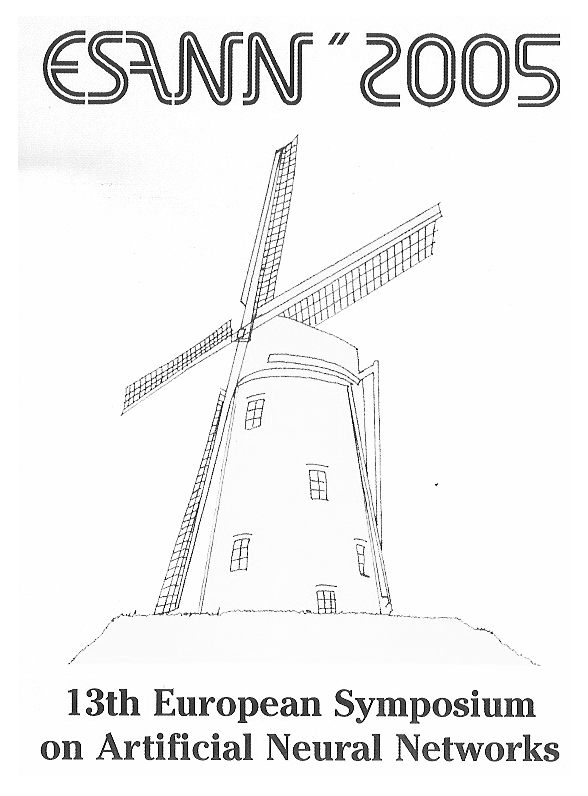
\includegraphics[scale=0.6]{ESANN2005BW.eps}
\caption{ESANN 2005: Announcement and call for
papers.}\label{Fig:MV}
\end{figure}

Table \ref{Tab:AgeWeight} shows an example of table.

\begin{table}[h!]
  \centering
  \begin{tabular}{|c|c|c|}
    \hline
    ID & age & weight \\
    \hline
    1& 15 & 65 \\
    2& 24 & 74\\
    3& 18 & 69 \\
    4& 32 & 78 \\
    \hline
  \end{tabular}
  \caption{Age and weight of people.}\label{Tab:AgeWeight}
\end{table}

\section{Citation}
This ESANNV2.tex file defines how to insert references, both for
BiBTeX and non-BiBTeX users.  Please read the instructions in this
file.

% ****************************************************************************
% BIBLIOGRAPHY AREA
% ****************************************************************************

\begin{footnotesize}

% IF YOU DO NOT USE BIBTEX, USE THE FOLLOWING SAMPLE SCHEME FOR THE REFERENCES
% ----------------------------------------------------------------------------
\begin{thebibliography}{99}

% For books
\bibitem{Haykin_book} S. Haykin, editor. \emph{Unsupervised Adaptive Filtering vol.1 : Blind Source Separation}, John Willey ans Sons, New York, 2000.

% For articles
\bibitem{DelfosseLoubaton_article}N. Delfosse and P. Loubaton, Adaptibe blind separation of sources: A deflation
approach, \emph{Signal Processing}, 45:59-83, Elsevier, 1995.

% For paper in proceedings published as serie books (LNCS,...)
\bibitem{CrucCichAmari_bookproceedings} S. Cruces, A. Cichocki and S. Amari, The minimum entropy and cumulants based contrast functions for blind source extraction. In J. Mira and A. Prieto, editors, proceedings of the 6$^{th}$ \emph{international workshop on artificial neural networks} ({IWANN} 2001), Lecture Notes in Computer Science 2085, pages 786-793,
Springer-Verlag, 2001.

% For paper in conference proceedings
\bibitem{VrinsArchambeau_proceedings} F. Vrins, C. Archambeau and M. Verleysen, Towards a local separation performances estimator using common ICA contrast functions? In M. Verleysen, editor, \emph{proceedings of the $12^{th}$
European Symposium on Artificial Neural Networks} ({ESANN} 2004),
d-side pub., pages 211-216, April 28-30, Bruges (Belgium), 2004.

% For Technical Report
\bibitem{Stone_TechRep} J. V. Stone and J. Porrill, Undercomplete independent component analysis for signal separation and dimension
reduction. Technical Report, Psychology Department, Sheffield
University, Sheffield, S10 2UR, England, October 1997.
\end{thebibliography}
% ----------------------------------------------------------------------------

% IF YOU USE BIBTEX,
% - DELETE THE TEXT BETWEEN THE TWO ABOVE DASHED LINES
% - UNCOMMENT THE NEXT TWO LINES AND REPLACE 'Name_Of_Your_BibFile'

\bibliographystyle{unsrt}
\bibliography{Name_Of_Your_BibFile}

\end{footnotesize}

% ****************************************************************************
% END OF BIBLIOGRAPHY AREA
% ****************************************************************************
\end{document}

\begin{table}[h!]
  \centering
  \begin{tabular}{|c|c|c|c|c|c|}
    \hline
    Training & Mean accuracy (\%) & Books & DVD & Electronics & KH \\
    \hline
    Books.t2 & 91 & 92 &  \\
    Books.t4 & 94 \\
    Books.t5 & 73 \\
    Dvd.t2 & 84 \\
    Dvd.t4 & 92 \\
    Dvd.t5 & 74 \\
    Electronics.t2 & 89 \\
    Electronics.t4 & 91 \\
    Electronics.t5 & 77 \\
    Kitchen housewares.t2 & 87 \\
    Kitchen housewares.t4 & 93 \\
    Kitchen housewares.t5 & 78 \\
    \hline
  \end{tabular}
  \caption{Results obtained with BART after training on books domain.}\label{Tab:bart_books}
\end{table}

\begin{table}[h!]
  \centering
  \begin{tabular}{|c|c|}
    \hline
    Training & Mean accuracy (\%) \\
    \hline
    Books.t2 & 92 \\
    Books.t4 & 95 \\
    Books.t5 & 73 \\
    Dvd.t2 & 86 \\
    Dvd.t4 & 92 \\
    Dvd.t5 & 74 \\
    Electronics.t2 & 88 \\
    Electronics.t4 & 90 \\
    Electronics.t5 & 78 \\
    Kitchen housewares.t2 & 86 \\
    Kitchen housewares.t4 & 93 \\
    Kitchen housewares.t5 & 77 \\
    \hline
  \end{tabular}
  \caption{Results obtained with BART after training on dvd domain.}\label{Tab:bart_dvd}
\end{table}


\end{document}
